\documentclass[11pt]{article}
\usepackage{latexsym}
\usepackage{amsmath}
\usepackage{amssymb}
\usepackage{amsthm}
\usepackage{epsfig}
\usepackage{graphicx}
\usepackage[tight]{subfigure}
% \usepackage{subcaption}
\usepackage{hyperref}

\usepackage{amsmath}
\usepackage{bbm}

\DeclareMathOperator*{\minimize}{min}
\DeclareMathOperator*{\maximize}{max}

\def\PP{\mathcal{P}}
\def\RR{\mathbb{R}}
\def\BB{\mathbb{B}}
\def\AA{\mathbb{A}}
\def\PP{\mathbb{P}}
\def\EE{\mathbb{E}}
\def\FF{\mathbb{F}}
\def\HH{\mathcal{H}}
\def\XX{\mathcal{X}}
\def\YY{\mathcal{Y}}
\def\NN{\mathbb{N}}
\def\TT{\mathcal{T}}
\def\DD{\mathcal{D}}
\def\SS{\mathcal{S}}
\def\LL{\mathcal{L}}
\def\MM{\mathcal{M}}
\def\err{\text{err}}
\def\ind{\mathbbm{1}}
\def\II{\mathcal{I}}
\def\ig{\mathcal{\gemini}}
\def\Lev{\textscl}


\usepackage{algorithm}
 %on linux you may need to run sudo apt-get install texlive-full to install algorithm.sys
\usepackage{algorithmic}

\usepackage{verbatim}

\newcommand{\handout}[5]{
  \noindent
  \begin{center}
  \framebox{
    \vbox{
      \hbox to 5.78in { {#1} \hfill #2 }
      \vspace{4mm}
      \hbox to 5.78in { {\Large \hfill #5  \hfill} }
      \vspace{2mm}
      \hbox to 5.78in { {\em #3 \hfill #4} }
    }
  }
  \end{center}
  \vspace*{4mm}
}

\newcommand{\lecture}[5]{\handout{#1}{#2}{#3}{#4}{#5}}
\newcommand{\collision}[0]{\mathrm{collision}}
\newcommand{\nocollision}[0]{\overline{\collision}}

\newcommand*{\QED}{\hfill\ensuremath{\square}}

\newtheorem{theorem}{Theorem}
\newtheorem{corollary}[theorem]{Corollary}
\newtheorem{lemma}[theorem]{Lemma}
\newtheorem{observation}[theorem]{Observation}
\newtheorem{proposition}[theorem]{Proposition}
\newtheorem{definition}[theorem]{Definition}
\newtheorem{claim}[theorem]{Claim}
\newtheorem{fact}[theorem]{Fact}
\newtheorem{assumption}[theorem]{Assumption}
\newtheorem{note}[theorem]{Note}

% 1-inch margins, from fullpage.sty by H.Partl, Version 2, Dec. 15, 1988.
\topmargin 0pt
\advance \topmargin by -\headheight
\advance \topmargin by -\headsep
\textheight 8.9in
\oddsidemargin 0pt
\evensidemargin \oddsidemargin
\marginparwidth 0.5in
\textwidth 6.5in

\parindent 0in
\parskip 1.5ex
%\renewcommand{\baselinestretch}{1.25}

\begin{document}

\lecture{Statistical Techniques in Robotics (16-831, S22)}{Lecture \#10
  (Monday, February 21, 2022)}{Lecturer: Kris Kitani}{Scribes: Michelle Zhao, Shane Deng}{Support Vector Machines}

\section{Review}
In the last lectures, we covered the algorithms of Gradient Descent, and Stochastic Gradient Descent (SGD). Gradient descent is an approach for minimizing convex, differentiable functions. Alternative gradient descent algorithms stochastically sample the data (SGD) or observe the data in mini-batches (Batch Gradient Descent), while maintaining convergence to the minimum solution. We observed how Stochastic Gradient Descent can be represented as an online convex optimization problem, and in particular, is a special case of Online Mirror Descent (OMD). 

%This section serves as a review of the previous lecture and any other context required to frame the content of the current lecture. 

%You may format the scribes in any way you like, aside from changing font style, size and page format. Please use subsections and paragraphs to increase the readability of your notes.

%Length requirement 1-2 pages.
        
\section{Introduction}
Online techniques can be very useful for supervised learning. In supervised learning, there is a distinct training stage where the parameters are determined. Then, in the testing stage, we leave parameters fixed, receive new data and make inferences on the new data.

Compared to supervised learning, online learning interweaves the training and testing steps. In online learning, there's two main steps: an update step where we learn our parameters, and a prediction step where we make an inference and get feedback from the environment. Some supervised learning algorithms can also be solved by using online learning methods.

\begin{figure}[H]
    \centering
    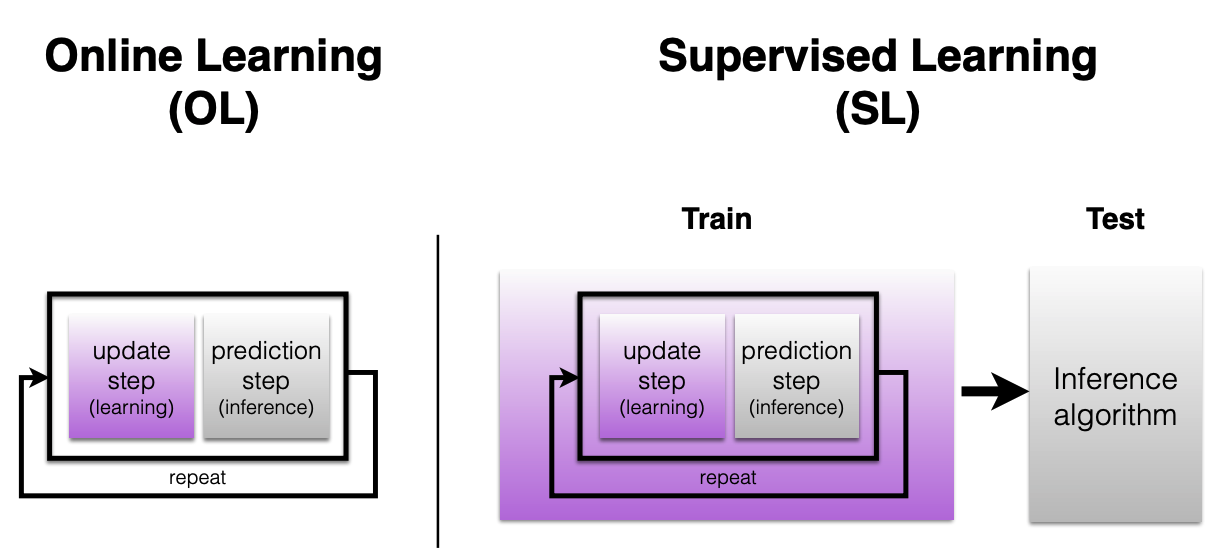
\includegraphics[width=0.5\textwidth]{images/sl_ol.png}
    \caption{Supervised learning can be solved using online learning methods.}
    \label{fig:sl_ol}
\end{figure}

In this lecture, we will focus on Support Vector Machines, an approach for classification with both an online learning and supervised learning interpretation.


\section{Online SVM}
\subsection{Convex Functions}
Recall from the previous lecture: \\
A function $f:S \rightarrow R$ is a convex function if it satisfies:
$$f(\alpha*w + (1-\alpha)*v) \leq \alpha*f(w) +(1-\alpha)*f(v) \; for \; all \; \alpha \in [0,1] $$
A key property is that the convex function has a global minimum which means it is suitable for optimization problems. 

\subsection{Hyperplanes}
In order to better understand the SVM algorithm, we first need to grasp the concept of hyperplanes. A hyperplane is a subspace whose dimension is $n-1$ of the main space. For example, in a 2D space (e.g a 2D surface), the hyperplane is a 1D line. More importantly, a hyperplane is a subspace that divides the data points into n sections. In the figure ~\ref{fig:sfig1}, a 2D plane separates the 3D points into 2 regions

\begin{figure}[H]
  \centering
  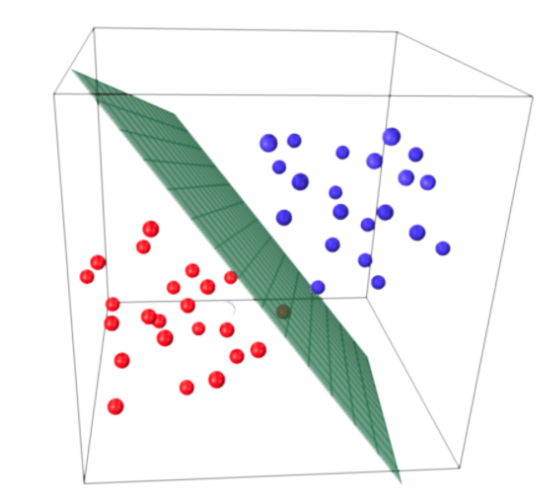
\includegraphics[width=.2\linewidth]{hyperplane.png}
  \caption{Hyperplane}
  \label{fig:sfig1}
\end{figure}

\subsubsection{Hyperplanes in 2D}
\begin{figure}[H]
  \centering
  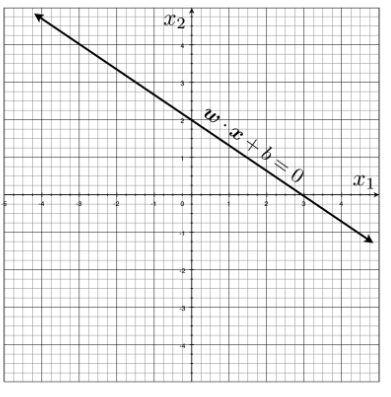
\includegraphics[width=.3\linewidth]{2Dplane.png}
  \caption{Hyperplane in 2D}
  \label{fig:sfig2}
\end{figure}

A standard representation of a line is $w_1 x_1 + w_2 x_2 + b = 0$. A line can be written as a dot product plus a bias.
$$w \cdot x + b = 0 \; \text{(offset\; / \;bias\; outside)}$$
$$w \in \RR^2 $$

Another version is the 3-dimensional version: add a weight 1 to the x vector, and push the bias inside of the weights.
$$w \cdot x  = 0 \;\text{(offset\; / \;bias\; inside)}$$
$$w \in \RR^3 $$

\textbf{Note:} An important property of this hyperplane is that you are free to choose any normalization you want on $\mathbf{w}$. You can multiply this side of the equation by any scalar $\lambda$. $\lambda$ can be anything and the equation still describes the same line.
 
$$w_1 x_1 + w_2 x_2 + b = 0$$
$$\lambda(w_1 x_1 + w_2 x_2 + b )= 0$$

$$w \cdot x + b = 0$$
\begin{itemize}
\item{
\textbf{Vertical distance between the origin and the hyperplane:} From the figure ~\ref{fig:sfig3}, perpendicular distance of the vector space to the origin is $\frac{b}{||w||}$ by using the following procedure:

\begin{enumerate}
    % \centering
    \item Scale $w \cdot x + b = 0$ by $\frac{1}{||w||}$.
    \item Use trigonometry to calculate the distance: $x*\cos{\theta} + y*\sin{\theta} = \rho$
    \item Then we can rearrange: $\rho = \frac{b}{||w||}$
    
\end{enumerate}

\begin{figure}[H]
  \centering
  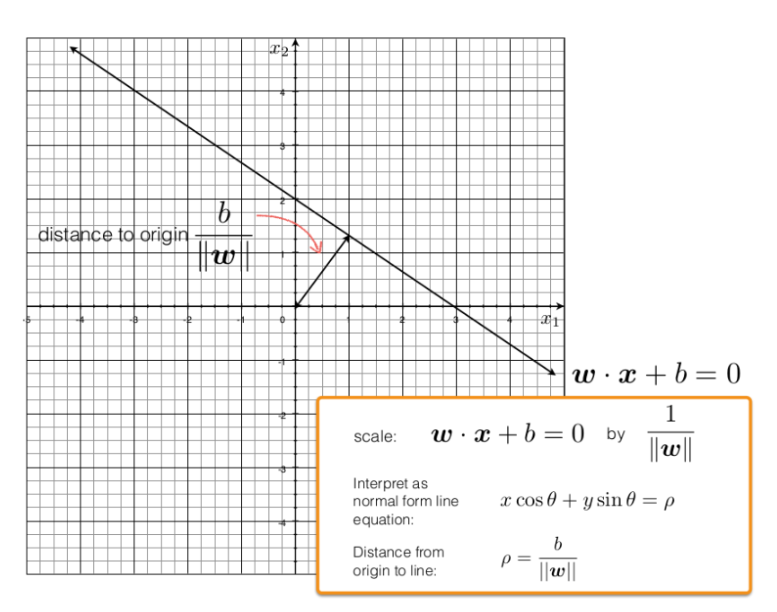
\includegraphics[width=.6\linewidth]{normal_distance.png}
  \caption{Normal distance between a hyperplane and the origin in 2D}
  \label{fig:sfig3}
\end{figure}
}

\item{
\textbf{Vertical distance between two parallel hyperplanes:} From the figure ~\ref{fig:sfig4}, perpendicular distance between one hyperplane and its adjacent hyperplane is $\frac{1}{||w||}$ assuming that the bias term is 1,  by using the following procedures:
\begin{enumerate}
    % \centering
    \item We know from the previous example that the perpendicular distance between the hyperplane and the origin is: $\frac{b}{||w||}$
    \item We shift the hyperplane upwards by 1, to $w \cdot x + b = -1$. We rearrange to get $w \cdot x + (b+1)= 0$. Using the formula for the perpendicular distance between the hyperplane and origin, we get that the distance from this line to the origin is: $\frac{b+1}{||w||}$.
    \item Hence, the pependicular distance between these two hyperplanes is $\frac{b+1}{||w||} - \frac{b}{||w||} = \frac{1}{||w||}$.
\end{enumerate}

\begin{figure}[H]
  \centering
  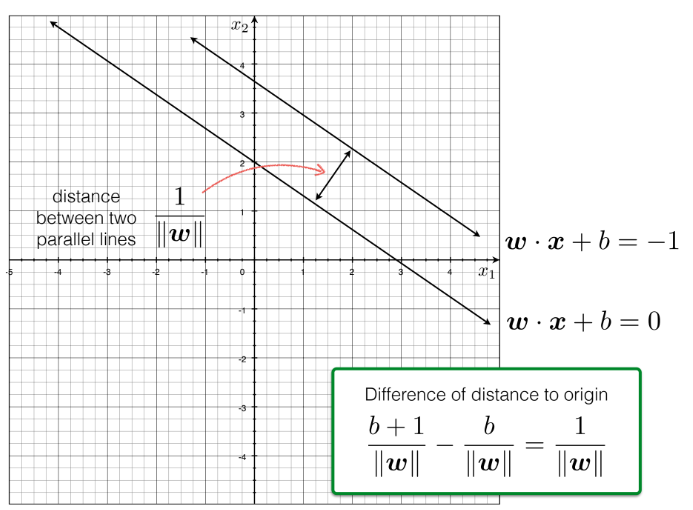
\includegraphics[width=.48\linewidth]{two_lines.png}
  \caption{Normal distance between two parallel hyperplanes in 2D}
  \label{fig:sfig4}
\end{figure}

}
\end{itemize}

\subsubsection{Hyperplanes (lines) in 3D}
We can extend this same idea to a higher dimension. For instance,a 3D plane will have the same equation but with different dimensions.The dimensions of a vector in 3D (outside bias form) is 3.

% \item{
\textbf{Vertical distance between two parallel hyperplanes:} From the figure ~\ref{fig:sfig5}, perpendicular distance between one hyperplane and its adjacent hyperplane is $\frac{2}{||w||}$ assuming that the bias term is at increment of 1( in this case, if we shift the plane in the +1 and -1 directions, the distance between the two of them is $\frac{2}{||w||}$.), by using the following procedures:
\begin{enumerate}
    % \centering
    \item Hyperplane ($w \cdot x + b = -1 \rightarrow w \cdot x + (b+1) = 0$) has distance from the origin of: $\frac{b+1}{||w||}$
     \item Hyperplane ($w \cdot x + b = 1 \rightarrow w \cdot x + (b-1) = 0$) has distance from the origin of: $\frac{b-1}{||w||}$
    \item Hence, the pependicular distance between these two hyperplanes: $\frac{b+1}{||w||} - \frac{b-1}{||w||} = \frac{2}{||w||}$
\end{enumerate}

\begin{figure}[H]
  \centering
  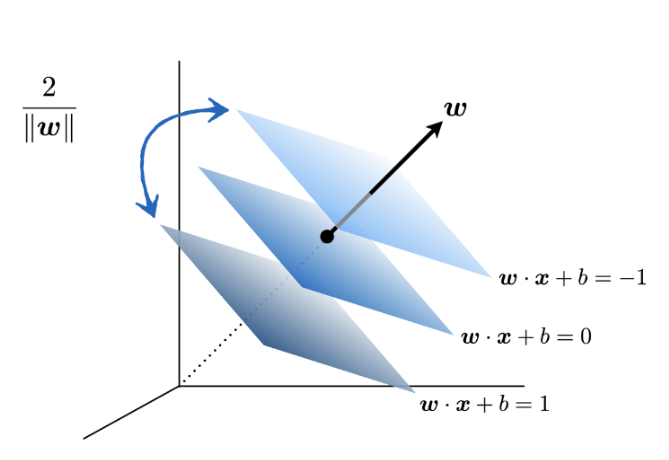
\includegraphics[width=.49\linewidth]{two_parallel.png}
  \caption{Normal distance between two parallel hyperplanes in 3D}
  \label{fig:sfig5}
\end{figure}

% }

\section{Support Vector Machine (Maximum-Margin Classifier)}
Consider a binary clasification problem in which we have some dataset $\DD$ containing data points of label $y \in \{1, -1\}$. Our task is to learn some decision boundary that best classifies this data. Assume that the data is linearly separable. There is an infinite set of possible separating hyperplanes for linearly separable data, but we want to learn a linear separator with as large of a margin as possible.

\begin{definition}[Support Vectors or Interior Points]
A support vector, or interior point, is the data point that lies closest to the hyperplane on each side of the decision boundary.
\end{definition}

\begin{definition}[Margin]
A margin ($\gamma$) is the distance between an interior point and the separating hyperplane. 
\end{definition}

\begin{figure}[H]
    \centering
    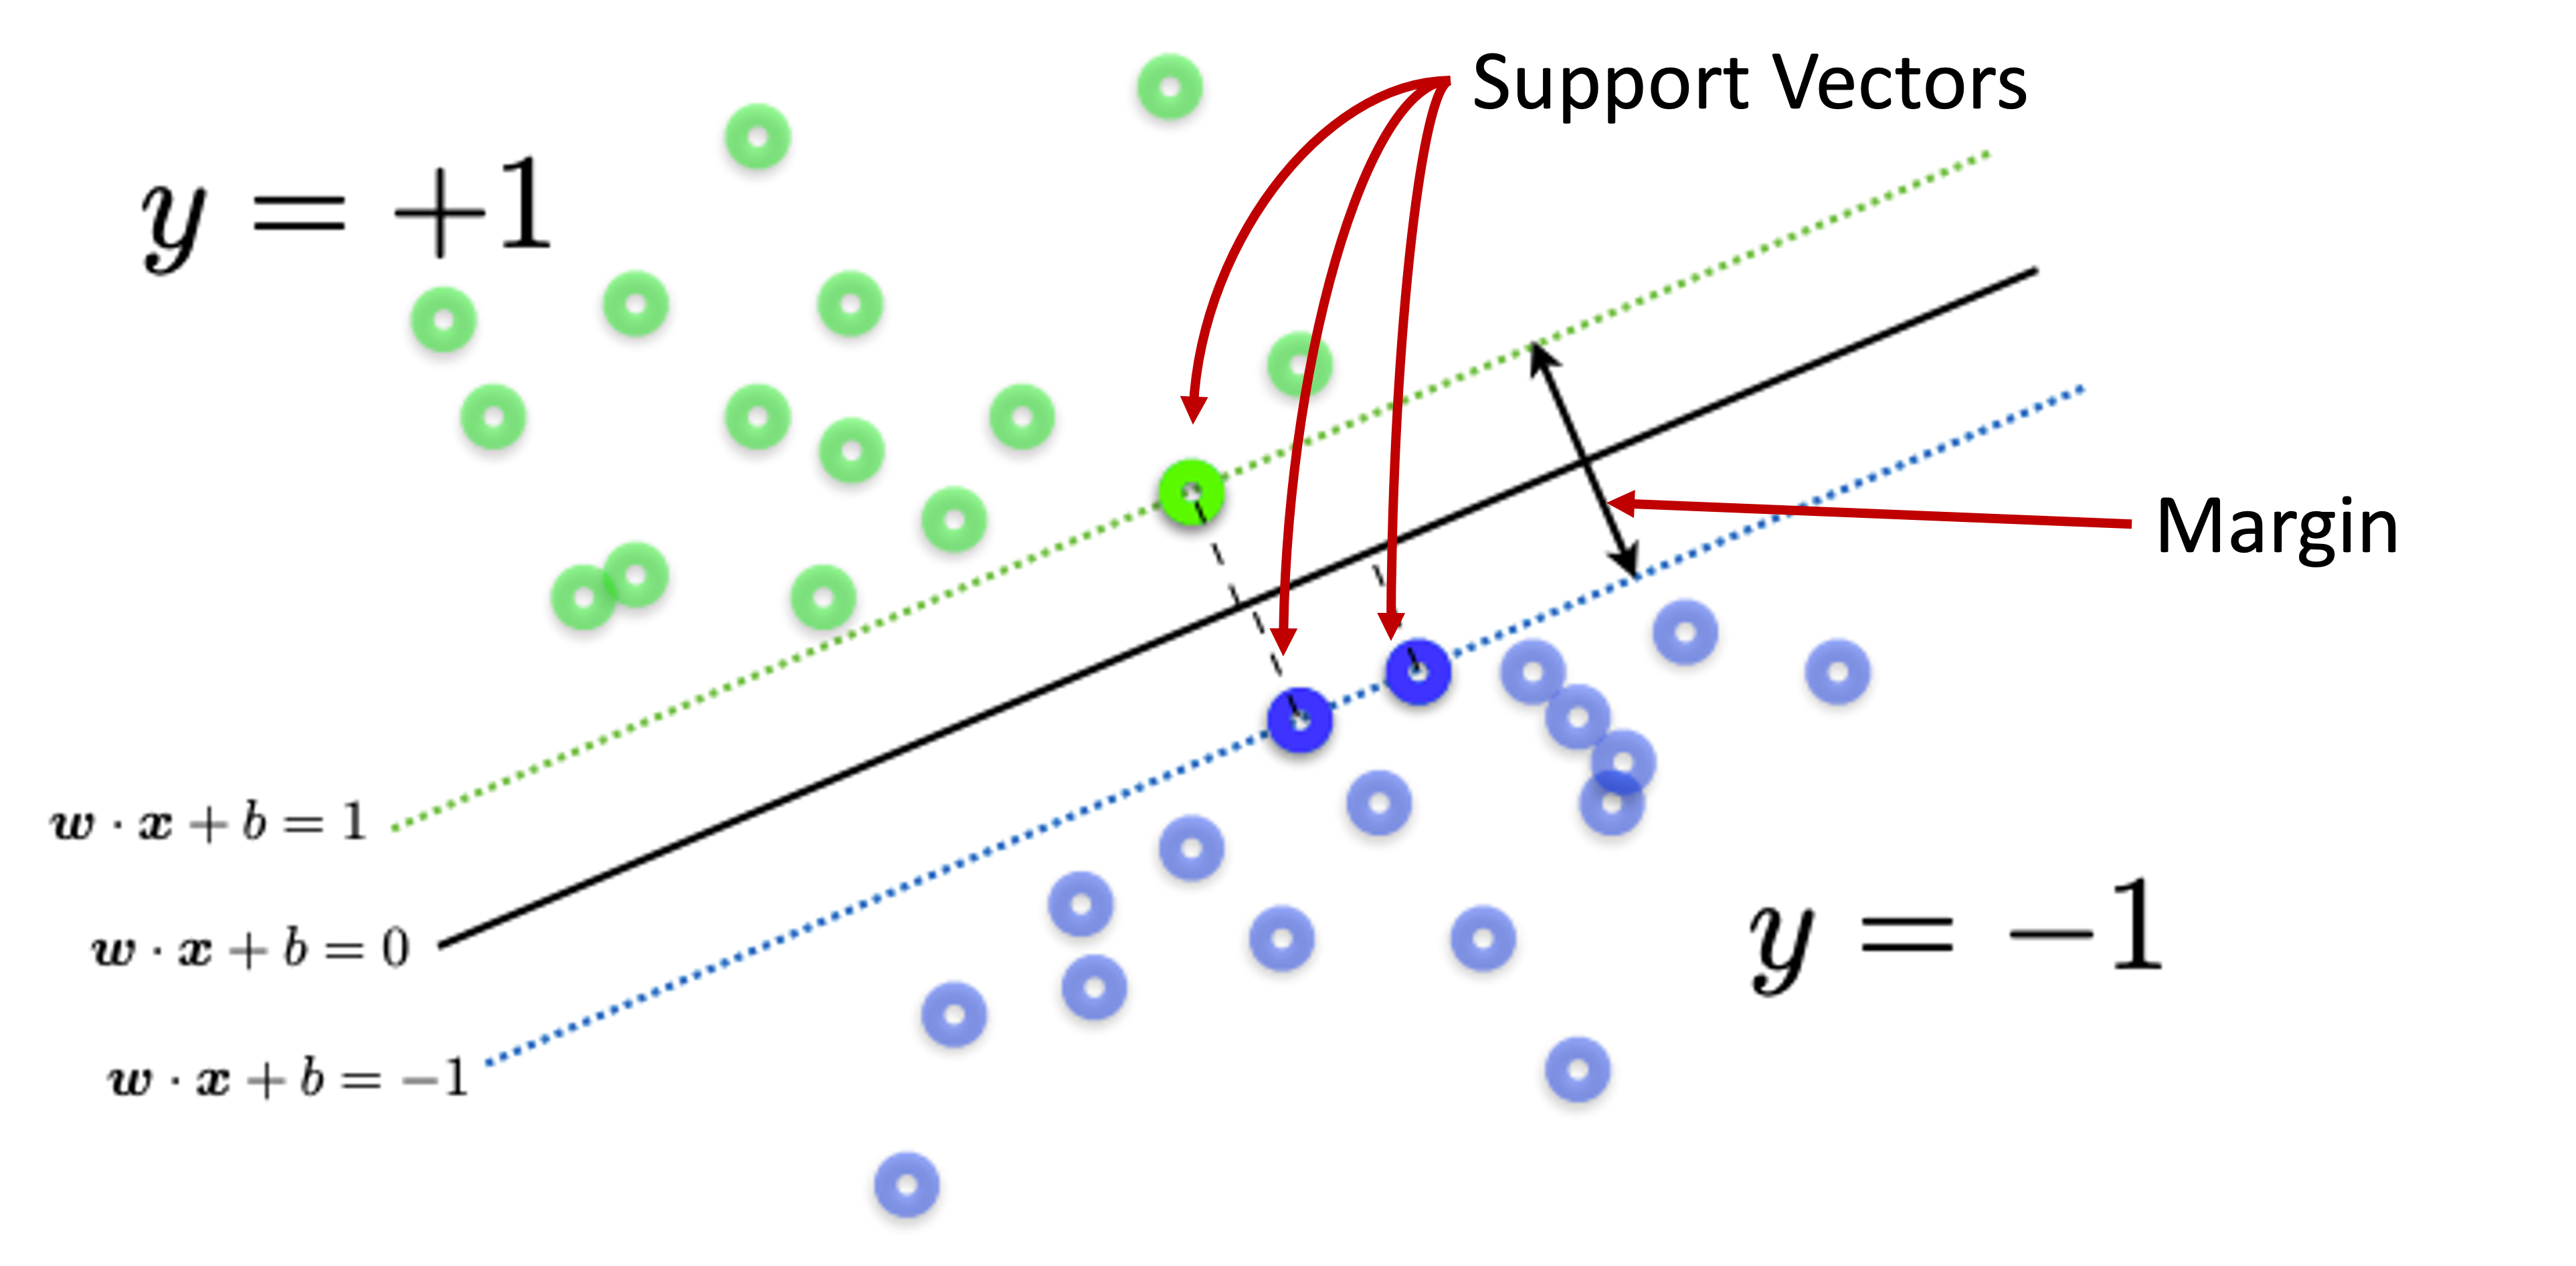
\includegraphics[width=0.6\textwidth]{images/support_vector.png}
    \caption{Support vectors are the points closest to the decision boundary, or separating hyperplane. The margin is the distance between support vector and hyperplane.}
    \label{fig:support_vectors}
\end{figure}

The objective is to find the separating hyperplane that maximizes the margin, $\gamma$ so that we can find a hyperplane that can most distinguish and separate the datesets, hence why it is called the Maximum Margin Solution. The maximum-margin classifier is also the most stable hyperplane to perturbations of data, meaning that if you were to move data points around slightly, the hyperplane would most likely remain valid under those small changes. The method is also called a Support Vector Machine (SVM).

\subsubsection{Hard SVM}
Recall that a hyperplane in 3D can be represented as $\mathbf{w} \cdot \mathbf{x} + b = 0$ whose distance to the origin is $\frac{b}{||w||}$. Shifting this hyperplane up by 1 gives us $\mathbf{w} \cdot \mathbf{x} + b = -1$ and down by 1 gives us $\mathbf{w} \cdot \mathbf{x} + b = 1$. The margin, or gap, between these two parallel hyperplanes is $\frac{b+1}{||w||} - \frac{b-1}{||w||} = \frac{2}{||w||}$. See Figure \ref{fig:support_vectors}.
\\\\
Therefore, our objective can be formulated as a maximization problem.
\begin{equation}
\begin{aligned}
\max_{\mathbf{w}} \quad & \frac{2}{||\mathbf{w}||}\\
\textrm{s.t.} \quad &
\begin{cases}
& \mathbf{w} \cdot \mathbf{x_{i}} +b \geq 1 \text{ if } y_i = 1 \\
&\mathbf{w} \cdot \mathbf{x_{i}} +b \leq 1 \text{ if } y_i = -1 \text{ for } i = 1,..., N   
  \end{cases}\\
\end{aligned}
\end{equation}

We can further formulate this as a minimization problem:
\begin{equation}
\begin{aligned}
\min_{\mathbf{w}} \quad & ||\mathbf{w}||^2\\
\textrm{s.t.} \quad &
 y_i(\mathbf{w} \cdot \mathbf{x_{i}} +b) \geq 1 \text{ for } i = 1, .., N\\
\end{aligned}
\end{equation}

By taking the reciprocal of the objective $\frac{||\mathbf{w}||}{2}$, we can change the problem into a minimization problem. We are able to drop the scalar and can add the square to $||\mathbf{w}||^2$, because the minimum point of the objective is the same when squared. The squared objective simply means that we are penalizing large values of $||\mathbf{w}||$ more.

This is a convex quadratic programming (QP) problem, since we are minimizing a quadratic objective with linear constraints. Thus, a unique solution exists to this problem. 

This minimization problem is known as the "Primal Formulation" of a linear SVM. The objective function is $\min_{\mathbf{w}}  ||\mathbf{w}||^2$. The constraints $y_i(\mathbf{w} \cdot \mathbf{x_{i}} +b) \geq 1 \text{ for } i = 1, .., N$ are known as "hard" constraints, because we assume separability of the data. Hence, this formulation is also known as the "Hard-Margin SVM". If there is noise in the dataset, or the data is non-separable, it may not be possible to satisfy all constraints. In the next section, we relax the linear separability assumption in the "Soft-Margin SVM."


% \begin{figure}[h]
% \centering
% \begin{subfigure}[t]{0.5\textwidth}
%   \centering
%   \includegraphics[width=.3\linewidth]{Hard SVM.png}
%   \caption{Hard SVM}
%   \label{fig:sfig6}
% \end{subfigure}%
% \begin{subfigure}[t]{0.5\textwidth}
%   \centering
%   \includegraphics[width=.3\linewidth]{Soft SVM.png}
%   \caption{Soft SVM}
%   \label{fig:sfig6}
% \end{subfigure}
% \end{figure}

\begin{figure}[H]
    \centering
    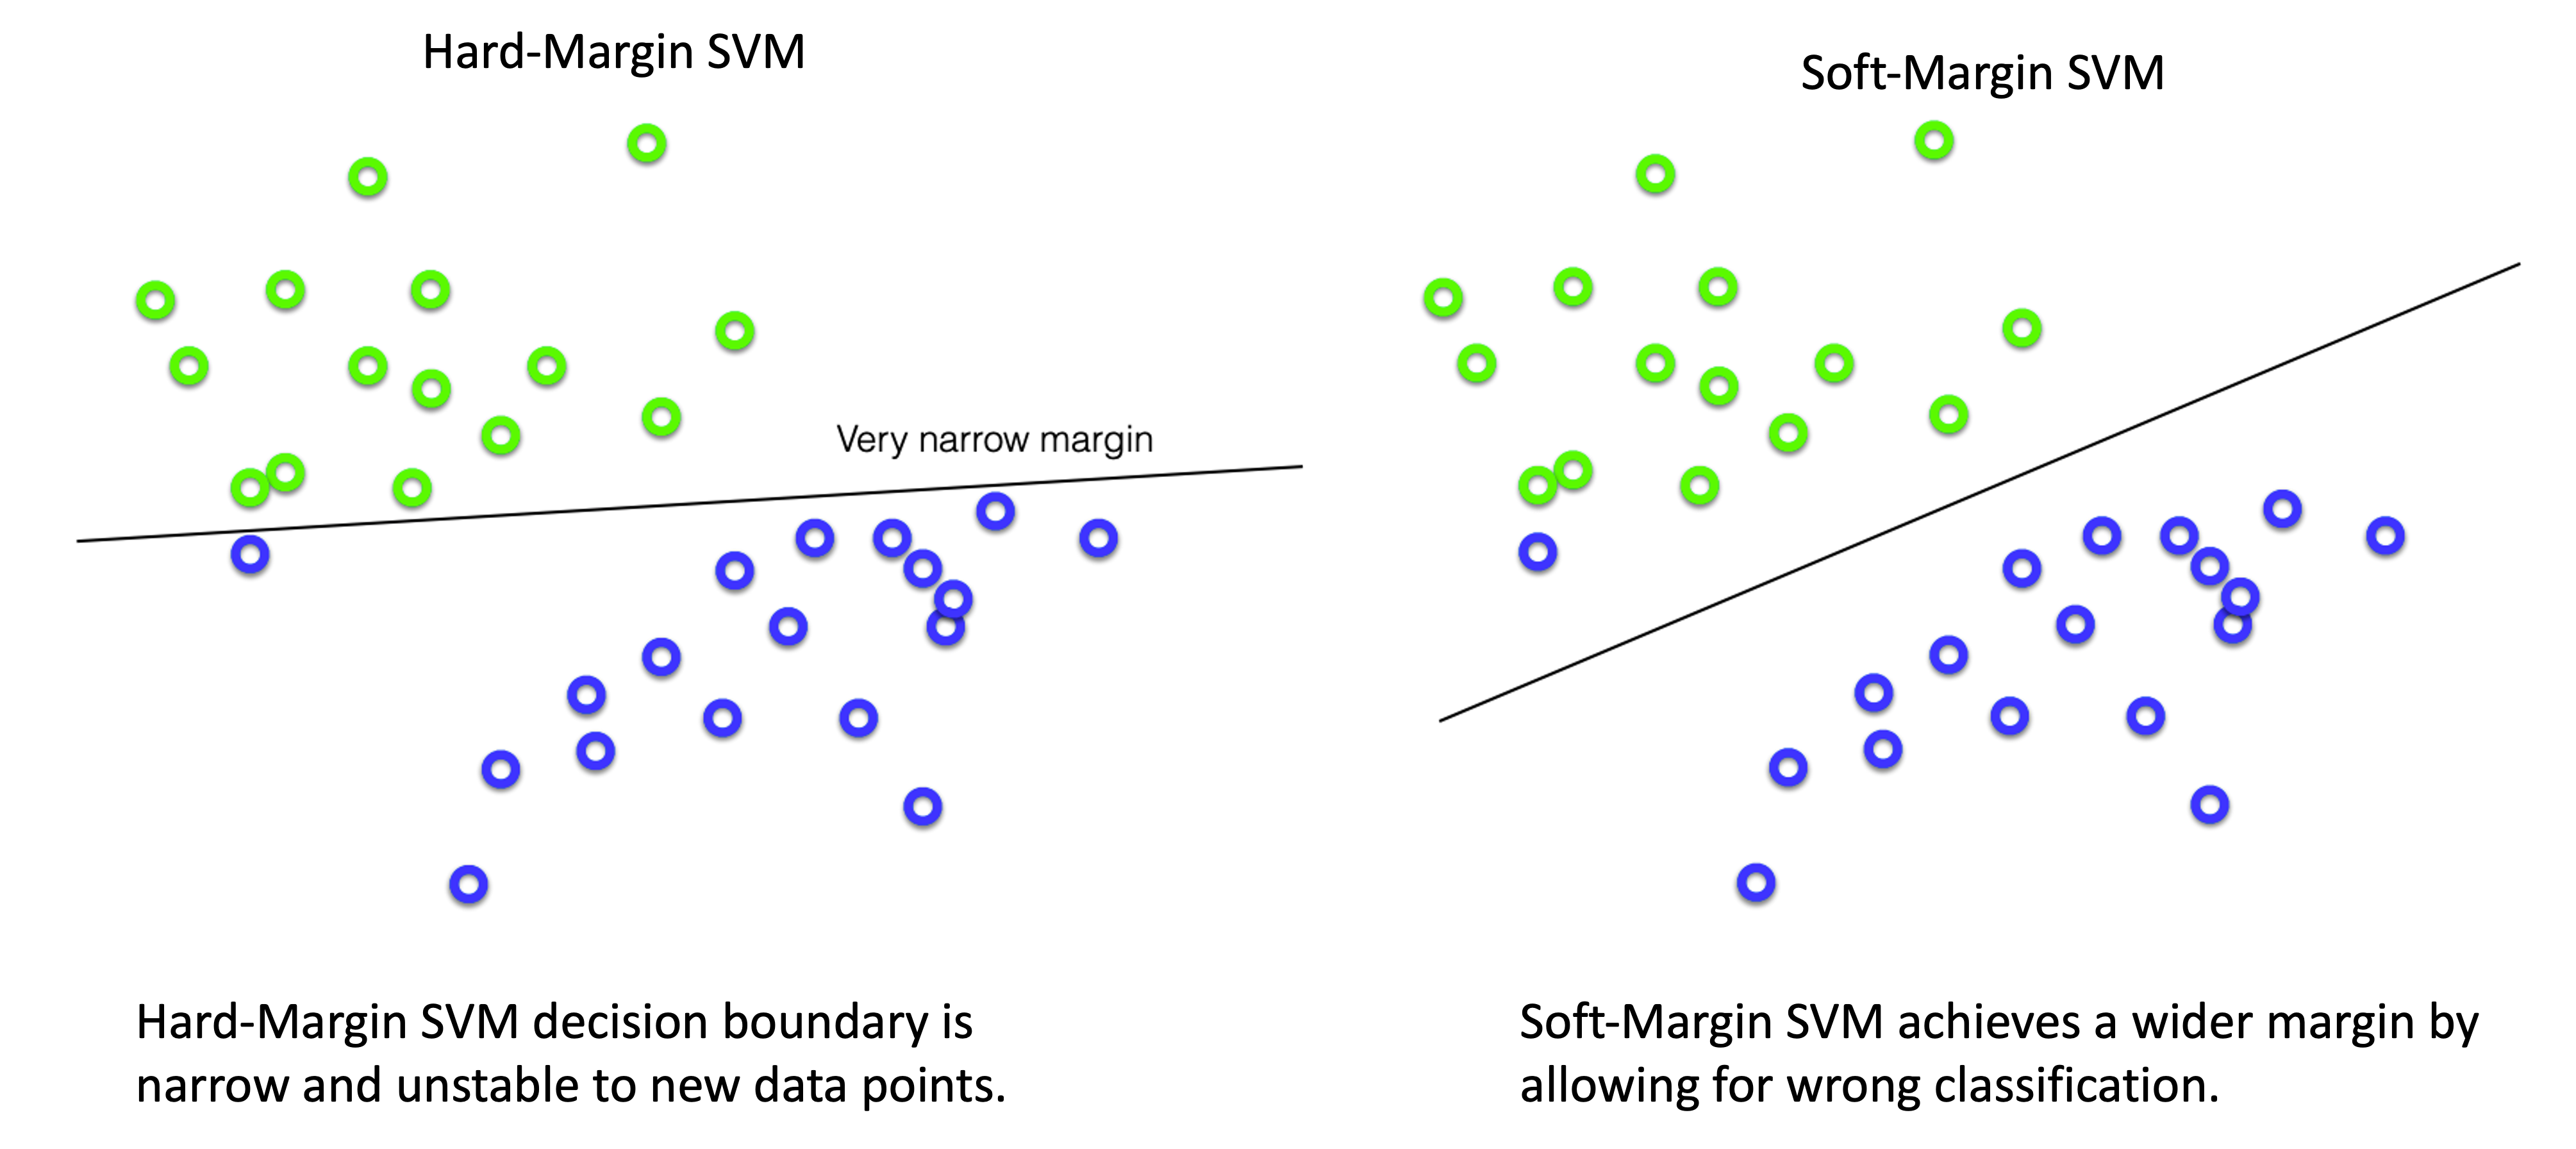
\includegraphics[width=0.8\textwidth]{images/hard_vs_soft.png}
    \caption{Hard-margin SVM achieves a narrow margin, but Soft-Margin SVM allows for a wider margin to be achieved.}
    \label{fig:hard_v_soft}
\end{figure}

\subsection{Soft-Margin SVM}
With Soft-Margin SVM, we relax the assumption that the data must be linearly separable. Soft-margin SVM is useful, because most real-world data is noisy, and a hard SVM classification on noisy data can result in very narrow margins that tend to be unstable. By allowing the classifier to make some mistakes, we can get a more stable decision boundary with larger margins. See Figure 7 and 8.
\subsubsection{Slack Variable}

Soft-Margin SVM introduces a slack constraint, which represents how mistake-tolerant the soft-margin SVM is. The slack variable, $ \xi_i$, geometrically, is the distance from a misclassified point to the margin corresponding to its true label. $\xi_i\geq 0$.

\begin{figure}[H]
    \centering
    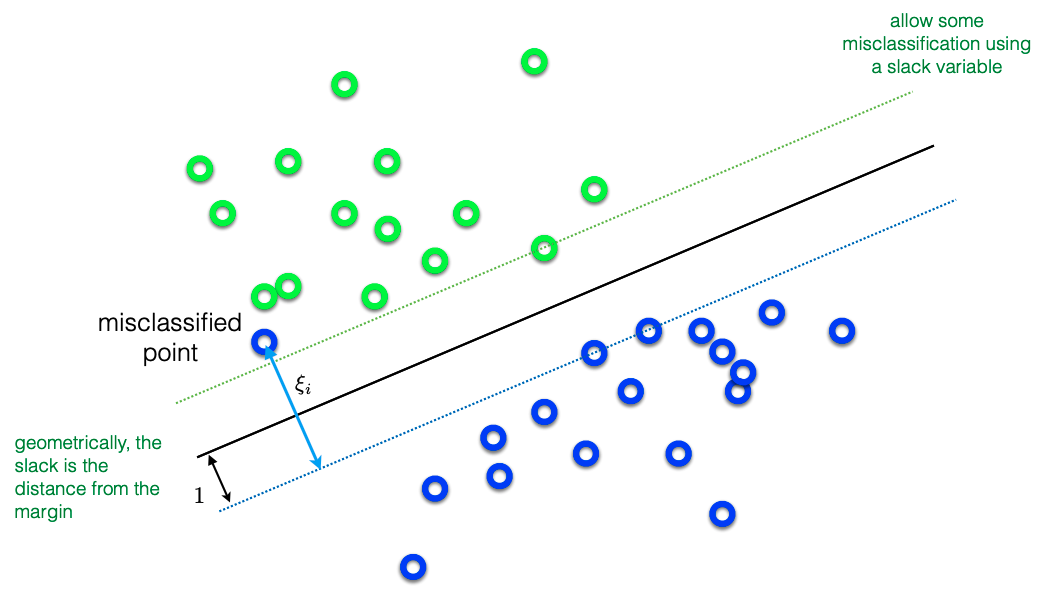
\includegraphics[width=0.6\textwidth]{images/slack_variable.png}
    \caption{The slack constraint allows the Soft-Margin SVM to make mistakes in order to achieve a larger margin. The constraint allows the algorithm to trade off between optimizing for a larger margin or more accurate classification.}
    \label{fig:my_label}
\end{figure}

In general, we want the slack variable to be as small as possible. A small $\xi_i$ allows for small mistakes to be made by the algorithm. Small mistakes are mistakes close to the decision boundary, and not far from the hyperplane corresponding to the true label. A large $\xi_i$ means that the SVM is allowing for large mistakes to be made.

\subsubsection{Soft-Margin SVM Objective}
In order to allow for some misclassification of the SVM, we can add $- \xi_i$ to the original hard-margin constraint, $y_i(w \cdot x_i + b) \geq 1$. The constraint becomes $y_i(w \cdot x_i + b) \geq 1 - \xi_i$. 

The Soft-Margin problem is thus formulated as:
\begin{equation}
\begin{aligned}
\min_{\mathbf{w}} \quad & ||\mathbf{w}||^2 + C\sum_i \xi_i \\
\textrm{s.t.} \quad &
 y_i(\mathbf{w} \cdot \mathbf{x_{i}} +b) \geq 1 -\xi_i \text{ for } i = 1, .., N\\
\end{aligned}
\end{equation}

Important notes on the soft-margin objective:
\begin{itemize}
    \item The slack variable allows for mistakes, as long as the inverse margin is minimized.
    \item Every constraint can be satisfied if slack is large. 
    \item C is a regularization parameter. If C is small, we do not prioritize keeping the slack small, and thus this results in large margins. If C is big, we prioritize keeping the slack small, and thus, we get a small margin. 
    \item This is still a quadratic programming (QP) problem since it still has a quadratic objective and linear constraints. Thus, we know that there exists a unique solution.
\end{itemize}



% \begin{figure}[h]
%     \centering
%     \begin{subfigure}{0.5\textwidth}
%       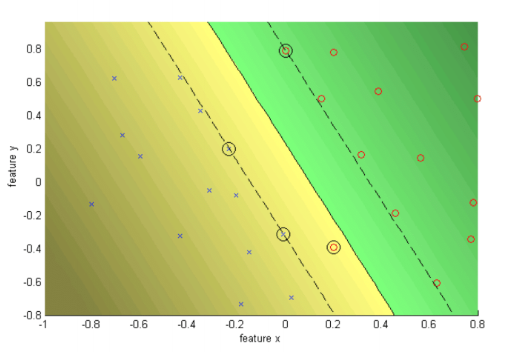
\includegraphics[width=.2\linewidth]{Soft Margin.png}
%       \caption{Soft}
%       \label{fig:sfig1}
%     \end{subfigure}%

%     \begin{subfigure}{0.5\textwidth}

%       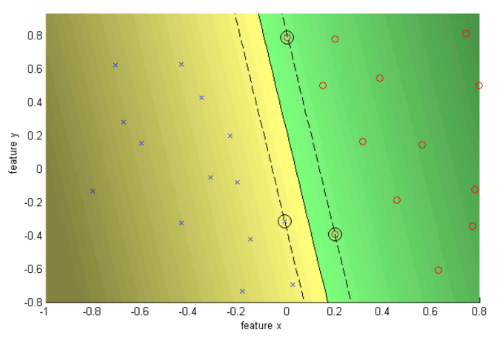
\includegraphics[width=.2\linewidth]{Hard Margin.png}
%       \caption{Hard}
%       \label{fig:sfig2}
%     \end{subfigure}
% \end{figure}


\subsection{Stochastic (Sub) Gradient Descent for Soft-Margin SVM Classifier}
In order to solve the Soft-Margin SVM, we will merge the linear constraints into the objective function.
We merge the bias term, $b$, into the weight vector, $\mathbf{w}$. We move the slack variable to one side of the optimization constraint inequality, and get $1 - y_i(\mathbf{w} \cdot \mathbf{x_{i}}) \leq \xi_i$. This term is then added to the objective, giving us
\begin{equation}
\begin{aligned}
\min_{\mathbf{w}} \quad & \frac{\lambda}{2}||\mathbf{w}||^2 + \frac{1}{N}\sum_{i=1}^N 1 - y_i \mathbf{w}^T \mathbf{x}_i \\
\end{aligned}
\end{equation}

The problem with this objective function is that the component $1 - y_i \mathbf{w}^T \mathbf{x}_i$ becomes is a very large negative value for "easy" data points that are correctly classified by a large margin, meaning the data points lie far from the separating hyperplane. For mistaken points, the value $1 - y_i \mathbf{w}^T \mathbf{x}_i$ is small, and is thus overpowered by large positive values of correct points.

\begin{figure}[H]
  \centering
  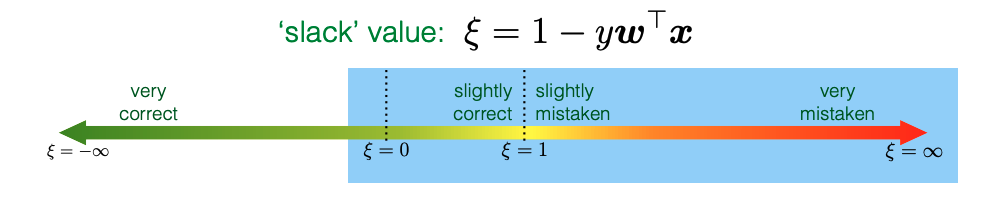
\includegraphics[width=.6\linewidth]{images/spectrum_highlight.png}
  \caption{We want to penalize the algorithm for mistakes, and weakly correct data points. We want to ignore "very correct" data, by focusing on the right hand side of this spectrum.}
  \label{fig:spectrum}
\end{figure}


As shown in figure ~\ref{fig:spectrum}, when the SVM classifies a data point "very" correctly, the slack variable is close to negative infinity. When it's highly mistaken, the slack variable is close to positive infinity. 
The portion of the spectrum we care about is the "slightly correct" to "very mistaken" part of the spectrum because we want to penalize mistakes and "weakly correct" data points to better optimize the parameters. The SVM should ignore "very correct" data because we don't want those points to influence the weight, $\mathbf{w}$ too much since they are already very correct. In other words, we don't want the correct points resulting in very large negative values to wash out the positive values from the mistaken points.

We use the Hinge loss to resolve this problem so that we only penalize for mistakes and weakly correct points (Figure ~\ref{fig:hinge})
% $$min_{w} \frac{\lambda}{2}||w||^2 + \frac{1}{N}\sum_{n}^M max\{0,1-y_n w^T x_n\}$$
\begin{equation}
\begin{aligned}
\min_{\mathbf{w}} \quad & \frac{\lambda}{2}||\mathbf{w}||^2 + \frac{1}{N}\sum_{i=1}^N \max\{0, 1 - y_i \mathbf{w}^T \mathbf{x}_i\} \\
\end{aligned}
\end{equation}

\begin{figure}[H]
  \centering
  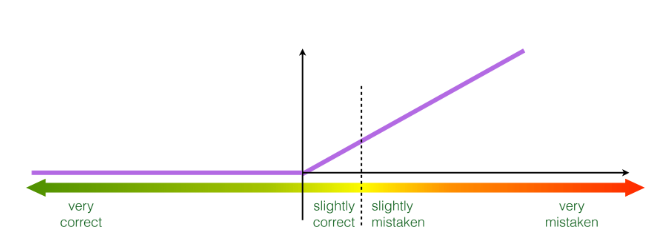
\includegraphics[width=.6\linewidth]{hinge.png}
  \caption{Hinge loss function to replace the original function}
  \label{fig:hinge}
\end{figure}

The regularization term $\frac{\lambda}{2}||w||^2$ is quadratic. The loss function is linear $ \frac{1}{N}\sum_{i}^N max\{0,1-y_i w^T x_i\}$. Therefore, this function is convex. \textbf{This is Online Mirror Descent with quadratic regularization and a piece-wise linear loss function.}

\textbf{Several Important Keypoints:}
\begin{itemize}
    \item The function is convex because it resembles the online mirror descent form with quadratic regularization and a piece-wise linear loss function.
    \item The function is not differentiable because the hinge has a kink point.
    \item We can not use gradient descent to solve the loss function because the function is not differentiable.
    \item We could use sub-gradient descent to optimize the function.
\end{itemize}

\subsection{Sub-gradients}
For a differentiable convex function, there's only one line that lower bound the function at any point.
For a non-differentiable convex function, there's many (infinite) lines that lower bound the function. These are called \textbf{subgradients}.

\begin{figure}[H]
  \centering
  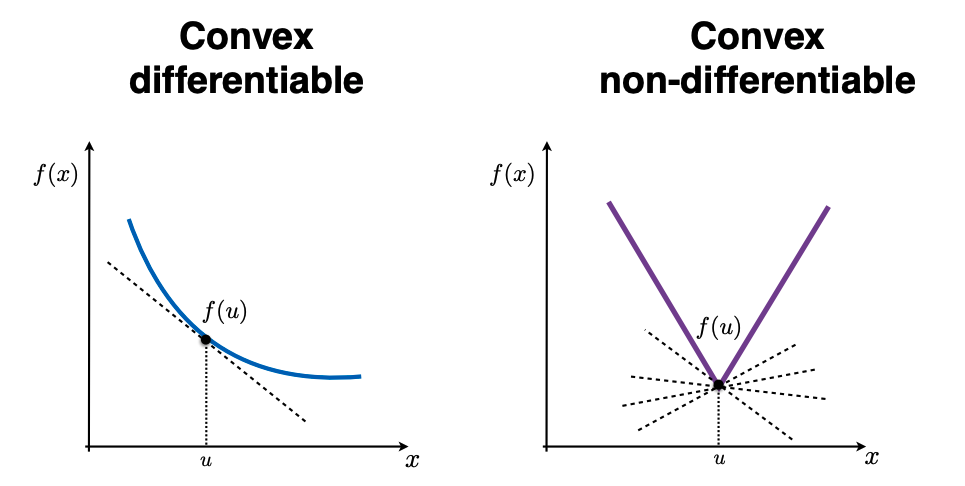
\includegraphics[width=.6\linewidth]{images/subgrads.png}
  \caption{Convex differentiable functions have one lower bound to the function at a given point, known as the gradient. Convex, non-differentiable functions has infinitely many.}
  \label{fig:subgrads}
\end{figure}

The hinge loss function is not differentiable. For the hinge loss function, there are many possible sub-gradients. 
We will use two subgradients:
\begin{equation}
  z_i =
    \begin{cases}
      0 & \text{if } y_i \mathbf{w}^T \mathbf{x}_i\\
      -y_i \mathbf{x_i} & \text{otherwise}\\
    \end{cases}       
\end{equation}

This piecewise subgradient states that if the SVM and observation label are in agreement, meaning there is sufficient distance from the hyperplane $\rightarrow y_i \mathbf{w}^T \mathbf{x}_i \geq 1$, then the gradient is 0. If the SVM classification is wrong, or is not sufficiently correct represented by $y_i \mathbf{w}^T \mathbf{x}_i \leq 1$, then the gradient is $-y_i \mathbf{x_i}$.

\begin{algorithm}[H]
\caption{Soft SVM}
\label{algo:SVM}
\begin{algorithmic}[1]
\STATE $\mathbf{w}^{(0)} \leftarrow 0 \in R^N$ \COMMENT{Written in OMD format} \hfill
\FOR{$t=0,\;\cdots,\;T-1$}
\STATE \textsc{Receive} ($\textbf y_d, x_d \sim D$) \COMMENT{Receive sample from environment (training data)} \hfill 
\STATE $\pmb{\theta}^t = \pmb{\theta}^{(t-1)} + y_d x_d \cdot \mathbbm{1}[y_d(\mathbf{w}^{(t)} \mathbf{x}_d) < 1]$ \COMMENT{Dual parameter update} \hfill
\STATE $\mathbf{w}^{(t+1)}\leftarrow \dfrac{1}{\lambda (t+1)} \pmb{\theta}^t$ \COMMENT{Mirror projection} \hfill
\ENDFOR
\end{algorithmic}
\end{algorithm}

We sample an observation-label pair from the dataset. Another way of thinking of this is receiving a data sample from an environment. We then perform the dual parameter update. The new parameter is the old parameter plus the gradient of the loss function. Next, we perform the mirror projection.

\subsection{Comparison of SoftSVM with Perceptron}
Recall the Perceptron algorithm written in the online mirror descent format.
\begin{algorithm}[H]
\caption{Perceptron Algorithm}
\label{algo:Perceptrom}
\begin{algorithmic}[1]
\STATE $\textbf{w}^{(0)} \leftarrow 0 \in R^N$ \COMMENT{Written in OMD format} \hfill
\FOR{$t=0,\;\cdots,\;T-1$}
\STATE \textsc{Receive} ($\mathbf{x}^{(t)}, y^{(t)}$) \hfill 
% \STATE $\hat{y}^{(t)}=h_i(\textbf{x}^{(t)})$ \COMMENT{this is a comment} \hfill
% \STATE \textsc{Receive} ($y^{(t)}\in\{-1, 1\}$) \hfill 
\STATE $\pmb{\theta}^{(t)} = \pmb{\theta}^{(t-1)} +y^{(t)} \mathbf{x}^{(t)} \cdot \mathbbm{1}[y^{(t)} \langle \mathbf{w}^{(t)}, \mathbf{x}^{(t)} < 0 \rangle] $ \COMMENT{Dual parameter update}\hfill

\STATE $\mathbf{w}^{(t+1)} =  \theta^{(t)}$ \COMMENT{Mirror projection} \hfill 
\ENDFOR
\end{algorithmic}
\end{algorithm}

SoftSVM and Perceptron both have piecewise loss functions due to both using hinge loss and quadratic regularization. In terms of the algorithm itself, SVM and Perceptron algorithm have a similar dual parameter update. SVM uses a soft margin, but Perceptron does not use a margin. As a result, the Perceptron algorithm does not try to push the data points away from a hyperplane, but simply says that data must lie on one side of the hyperplane. The two algorithms also have a similar mirror function.


\section{Summary}
In this lecture, we covered hyperplanes and the geometry of a linear classifier. The SVM algorithm tries to classify all of its datapoints on the correct side of a separating hyperplane while maximizing the margin between the data and the hyperplane. Soft-margin SVM relaxes the assumption of linear separability and allows for a tradeoff between classification accuracy and margin width. Soft-margin SVM can be solved with Online Sub-gradient Descent.

\section{Appendix}
\subsection{Kernels and Non Linear SVM}
In the class, we mostly explored the case of linear separable datasets. While soft SVM could handle some non-linear datasets with some outliers, it usually performs very poorly when the datasets are strictly non-linear. For example, in figure ~\ref{fig:nonlinear}, we can see that the SVM algorithm performs very poorly on this dataset. 
\begin{figure}[H]
    \centering
    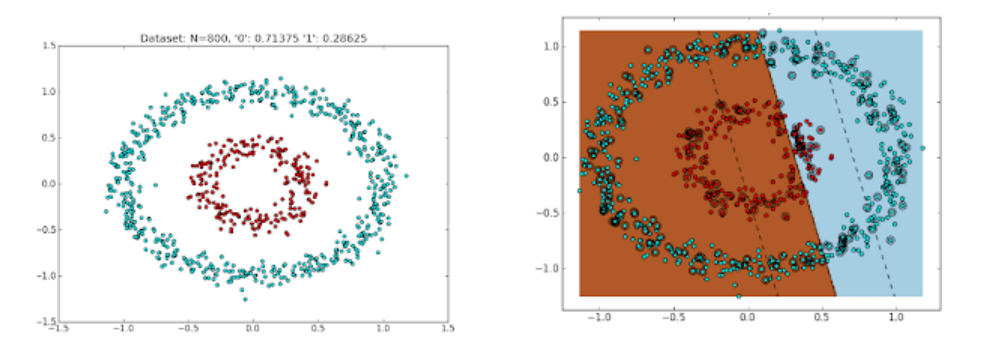
\includegraphics[width=0.6\textwidth]{images/nonlinear.png}
    \caption{Linear SVM on non-linear datasets.}
    \label{fig:nonlinear}
\end{figure}
In general, there are two methods to resolve this problem. (1) project the dataset to higher dimension or (2) use an non-linear kernel
\subsubsection{Higher dimension projection}
For instance, if we have the original dataset in 2D, we could perform the mapping $X^2 \rightarrow \{x^3,x^2\}$. Then the dataset might be separable in this new 3D space. As we see in the figure ~\ref{fig:projection}, the data is non-linear in 2D but can be linearly separated in 3D. \\
\textbf{Note: This will greatly increase the computation cost. As our datasets are getting more complex, projecting such datasets into higher dimension might not be computationally feasible }
\begin{figure}[H]
    \centering
    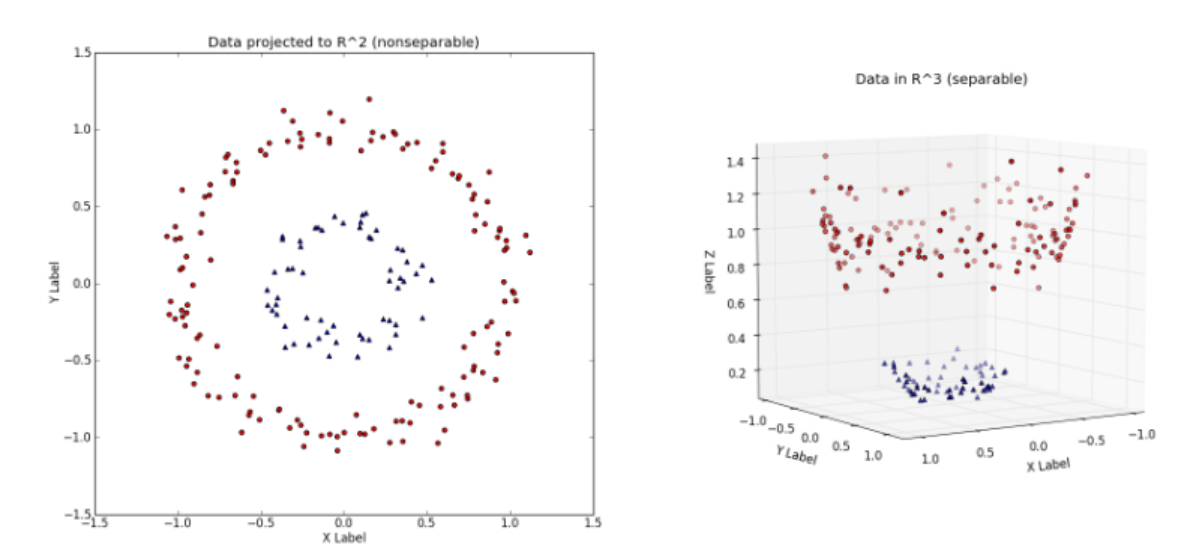
\includegraphics[width=0.6\textwidth]{images/projection.png}
    \caption{Data projection into a higher dimension.}
    \label{fig:projection}
\end{figure}

\subsection{Kernel tricks}
Kernels are essentially the functions that transform the features and weights into a way to split the data (How similar they are) or in other words, they are the tools that SVM uses to reason about the dataset\\

Common kernels are linear(which is the one we used), non-linera kernel, polynominal kernel, sigmod kernel, etc. 
For instance, if we apply non linear kernel as seen in figure ~\ref{fig:kernel}, we could get non-linear hyperplanes that could better separate the dataset 
\begin{figure}[H]
    \centering
    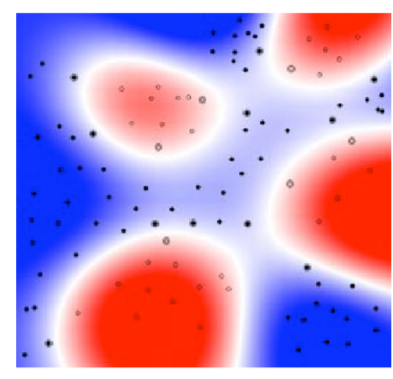
\includegraphics[width=0.5\textwidth]{images/kernel.png}
    \caption{Nonlinear rbf Kernel}
    \label{fig:kernel}
\end{figure}
\section*{References}
[1] Andrew Ng. CS229 Lecture Notes, Stanford. \url{https://see.stanford.edu/materials/aimlcs229/cs229-notes3.pdf}

[2] Tendolkar, G. (n.d.). 2.1.6 kernels and non linear SVM - Machine Learning Notebook. Google Sites. Retrieved February 22, 2022, from https://sites.google.com/site/machinelearningnotebook2/classification/binary-classification/kernels-and-non-linear-svm 

[3] R. Berwick, SVM Lecture Notes, MIT .http://web.mit.edu/6.034/wwwbob/svm-notes-long-08.pdf

%Include your references here. Please cite any resources you found useful.	
%Populate the refs.bib file or list your references manually. Be consistent in formatting!
{
\bibliography{refs}
\bibliographystyle{abbrv}
}

%\section{Appendix}
%This section provides any relevant background material that was not covered in the lectures, but was found to be useful for understanding the material. 
%For example, derivations, theory underlying techniques employed, etc. 

%Additionally, this section can summarizes applications or extensions of these techniques found in the literature. 

\end{document} % Done!


